\documentclass[10pt,conference,compsocconf,letterpaper]{IEEEtran}

\makeatletter
\def\ps@headings{%
\def\@oddhead{\mbox{}\scriptsize\rightmark \hfil \thepage}%
\def\@evenhead{\scriptsize\thepage \hfil \leftmark\mbox{}}%
\def\@oddfoot{}%
\def\@evenfoot{}}
\makeatother

\pagestyle{headings}
\usepackage{graphicx}
\usepackage[noadjust]{cite}
\usepackage{tabularx}
\usepackage{times}
\usepackage{alltt}
\usepackage{verbatim}
\usepackage{moreverb}
\usepackage{amsmath}
\usepackage{amssymb}
\ifCLASSINFOpdf \else \fi
\usepackage{url}
\usepackage{epsfig}
\usepackage{subfigure}
\usepackage{multirow}
%\usepackage{slashbox}
\usepackage[ruled,vlined]{algorithm2e}
\usepackage{mathrsfs}
\usepackage{amsthm}

\usepackage{dsfont}
\usepackage{cases}

\newtheorem{theorem}{Theorem}
\newtheorem{definition}{Definition}
\newtheorem{Lemma}{Lemma}

\newcommand{\ie}{{\em i.e.}}
\newcommand{\eg}{{\em e.g.}}
\newcommand{\et}{{\em et al.}}
\newcommand{\st}{{\em s.t.}}

\begin{document}

\title{Effective RSS data procurement for Crowdsensed Fingerprints for Indoor Localization}

%
%\author{\IEEEauthorblockN{Shitao Li$^1$,Xinyu Wu$^2$,Yucheng Yang$^2$,Wenxin Li$^2$, Xiaohua Tian$^{2,3}$, Xinbing Wang$^{1,3}$}
%\IEEEauthorblockA{
%1. Department of Mathematics, Shanghai Jiao Tong University, China\\
%2. Dept. of Electronic Engineering, Shanghai Jiao Tong University, China\\
%3. National Mobile Communications Research Laboratory, Southeast University, China}
% \{list12356, xtian, xwang8\}@sjtu.edu.cn}
%

\maketitle



\begin{abstract}
Crowdsourcing is currently one of the most prevailing methodology used in the received signal strength (RSS) fingerprinting based Indoor localization. The quality of the RSS data collected from the crowds is crucial to the accuracy of the localization system. While efforts have been dedicated to the incentive mechanism to acquire the data for the crowdsourcing platform, the problem that how to judge whether the data we should use and how to economically get access to these data that we want still remains unknown.  In this paper, we give a quantitative measurement of the quality of data through the probabilistic model and propose a pricing mechanism to economically acquire the data given a limited budget under the basic framework of online machine learning. Our mechanism achieves the best performance in data purchasing than the state of the art method. And we further gives the theoretical analysis of the best quality of the data we can get access through the purchasing mechanism. Moreover, we give the alternative best money-saving strategy when the quality of data is required.
\end{abstract}


\section{Introduction}\label{sectionintro}

\subsection{Indoor localization}
The past decade has witnessed a flourishing of indoor localization systems based on wireless techniques \cite{ rsscsi}, where the fingerprinting based methodology has been widely adopted due to its convenient deployability \cite{ mobicom04, horus }. The fingerprinting based indoor localization system has two phases: In the offline phase, the site surveyor observes the received signal strength (RSS) of Wi-Fi access points (APs) termed as RSS fingerprints at each reference point, and submit the fingerprints and the location information of the reference point to the localization database; in the online phase, a user needs localization service could submit the observed fingerprints to the database, which then returns the location of the reference point that matches the fingerprints best as the estimated location of the user.

The fingerprinting based method utilizes Wi-Fi APs widely existing in buildings and has no need for other dedicated infrastructure; however, the site survey in the offline phase requires substantial efforts, which is hardly accomplished by any single entity. The recent advances of fingerprinting localization systems utilize mobile crowdsensing approach to collect fingerprints \cite{ wen2015fundamental, Chenshu14, luo2014piloc, shen2013walkie, ez10, Chintalapudi10}. Mobile crowdsensing is a cost-effective approach to collect large scale data for mobile applications, where individuals with hand-held mobile devices collectively contribute sensing data so that information of certain events could be retrieved \cite{ganti2011mobile, han2016posted}. Although sensing participants could receive certain rewards for the efforts and resources spent on the sensing activity, the cost of mobile crowdsensing is still much lower than deploying the dedicated sensing networks \cite{ganti2011mobile}.

As the crowdsensing data are collected by unprofessional participants with non-dedicated equipment, the sensing data obtained are usually with considerable noise. The quality of the sensing data is the crux for evaluating contribution of the participants, which is the vitally important for effective utilizing rewards to incentivize participants to accomplish sensing tasks satisfactorily. However, how to evaluate the quality of the crowdsensing data is a challenging issue, because there is no ground truth for the collected data to be compared with. Efforts have been made to evaluate the crowdsensing data quality \cite{kawajiri2014steered}, and the task allocation scheme \cite{ cheung2015distributed, reddy2010recruitment}. and incentive mechanisms considering the data quality are proposed.

While the efforts have been made for quality-driven incentive mechanism \cite{lbs2,jin2015quality,peng2015pay,gao2015providing}, the state of the art method for crowdsensing data collection still focus on the incentive of workers. The economical problem is considered in \cite{peng2015pay}, however, the budget of the platform and is not included. Besides, all the work listed above do not consider the situation when data is coming in a sequential order and only
available in each round. How to acquire the high-quality data that is in a sequential order given the limited budget is still not fully investigated, which is the focus of this work. Our motivation is two-fold. On one hand, the existing work for sequential data procurement in the literature \cite{abernethy2015low}do not work well for the situation of indoor localization; on the other hand, we want to build a concrete measurement of RSS data specifically for the active learning mechanism. 

%the target of the paper
%pricing mechanism -> better RSS data -> better location precision
In this paper, we propose a pricing mechanism that can get higher quality of RSS data within limited budget. Using the high quality data we procure, the localization system could set a localization with higher accuracy. Our contributions are as following.


%the contribution and challenge
\begin{itemize}

\item  We design an effective way to measure the what kind of RSS data should we purchase. In most cases, the collected RSS data is not idealy in the exact position, to design an effective way to measure the impact of those imperfect data is crucial to our system. We make a thorough analysis of the impact that imperfect data may exert on the result of localization through the  probability model. 

\item We give the pricing strategy for the mechanism to acquire the high quality data. The mechanism has a theoretically better performance than the classical one proposed in \ref{}. The mechanism is robust in most indoor-localization situations, even the prior knowledge of the costs is not well understood and the noise in the crowdsensing data is rather arbitrary. 

\end{itemize}

The remaining of the paper is organized as following. The system structure and settings are given in section \ref{sysmodel}. The measurement of the RSS data quality is presented in Section \ref{loss}. Section\ref{probdef}  gives the abstract definition for the online data procurement mechanism. Section \ref{mainsolution} presents a pricing mechanism for the RSS data procurement to get the data with best quality give the limited budget. Section \ref{mainsolution} presents an alternative senario for the mechanism to achieve the least purchasing cost when the quality of data is given. Section \ref{exp&sim} gives our simulations and experiments for the mechanism we given before.



%\section{Related Work \label{sectionrelatedwork}}
%\subsection{Fingerprinting based Indoor Localization}
%The RSS Fingerprinting based . The early technique,'nearest neighbour(s) in signal space'(NNSS) \cite{radar},outputs the location with minimum Euclidean distance between RSSes stored in the database and RSSes measured as the estimation of the user’s location. However, NNSS still dangles the possibility of accuracy enhancement in that it fails to realize the joint location estimation from multiple APs \cite{castro01}. In order to take advantage of these multiple APs, Chintalapudi \emph{et al.} bring up an algorithm entitled as EZ localization, whose main contribution occurs in estimating mobile devices without any pre-deployment support of multiple APs \cite{Chintalapudi10}. EZ will learn from those acquired fingerprints, which reflect the value of mean and standard deviation of the RSSes corresponding to different APs, during the collection phase. Wen \emph{et. al} made a thorough study of the 
%
%\subsection{incentive mechanism for  Indoor Localization}
%Fingerprinting based Indoor localization requires largePeng \emph {et al.} %point out the deficiency induced by continuous data with poor quality to the preciseness and availability of services predicated on crowdsensing in conventional incentive mechanism designing, and they
%bring up an incentive mechanism both stimulating data provision and ensuring high quality \cite{Peng2015Pay}. Jin \emph{et al.} introduce a key metric, quality of information(QoI), which generally evinces the quality of users’ sensory data%but whose definition varies among different applications
%\cite{Jin2015Quality}. Taking QoI into consideration, the incentive mechanism can acquire data with higher quality making for further study like better identification for problems of medical devices \cite{Jin2015Quality}.\\

\section{Related Work \label{sectionrelatedwork}}

\subsection{Indoor localization with crowdsourcing}

%During the inception of indoor localization research in the context of WLAN, the technique to deduce a user's location is called 'nearest neighbour(s) in signal space'(NNSS) , whose marrow is calculating the Euclidean distance between RSSes stored in the database and RSSes measured during localizing, with the location minimizing that distance output as the ultimate estimation of the user’s location \cite{radar}. However, NNSS still dangles the possibility of accuracy enhancement in that it fails to realize the joint location estimation from multiple APs \cite{castro01}.

%In order to take advantage of these multiple APs, Chintalapudi \emph{et al.} bring up an algorithm entitled as EZ localization, whose main contribution occurs in estimating mobile devices without any pre-deployment support of multiple APs \cite{Chintalapudi10}. EZ will learn from those acquired fingerprints, which reflect the value of mean and standard deviation of the RSSes corresponding to different APs, during the fingerprint collection phase. %The key point of EZ is that it is erected on the fact that the physics of wireless propagation constrain the fingerprints reported to the server, and it models these constraints and couples them with a genetic algorithm to get the final solution.

In fingerprinting based indoor localization, one of the common approaches to collect fingerprints is crowdsourcing, in which any user with a mobile device like smart phone can acquire data while walking freely, without the requirement for users to have any technical training \cite{}. Wu \emph{et al.} design a localizing system LiFS, combining indoor localization with crowdsourcing and bypassing the conventional site survey process \cite{yang2012locating,wu2015smartphones}. They initially place several landmarks in the physical space, and then harness information from user motions and pinned sensors in smart phone to set up a sample space with high dimension, with which approximates the user's location. %The materialization of this sample space relies on Multidimensional Scaling(MDS) algorithm, visualizing the information of similarities and dissimilarities concealed in data \cite{Yang12}. Meanwhile, since the high-dimensional space generated by MDS can be applied to characterize the physical space as well, the estimation of a user’s location can be derived via comparing physical space and sample space with high dimension.
%More utilization of crowdsourcing method has been revealed.
%Rai \emph{et al.} develop a system called Zee \cite{Rai12}. %which denotes that no explicit effort on the part of users is needed
%While a mobile device is traversing indoors scanning Wi-Fi signals, Zee leverages inner sensors of the device to track the device itself.
Moreover, Shen \emph{et al.} present a crowdsourcing based system \emph{Walkie-Markie} \cite{walkie} to generate indoor pathway maps from the user contributed data. %The central idea of the system is to exploit Wi-Fi-Marks defined by Wi-Fi RSS features in the indoor space, so that crowdsourced data can be fused.
and Luo \emph{et al.} propose a self-calibrating participatory indoor localization system \cite{luo2014piloc}, which requires no prior knowledge about the building and user intervention including the floor planning. %Additionally, Crowdsourcing approach has also been applied to various domains such as transportation \cite{transportation2}, environment surveillance \cite{environment, environment2} and location based service \cite{lbs,Wen2015Quality}.

Nevertheless, the above work has not placed a premium on the fingerprint procurement phase. %just concluding this procedure as crowdsourcing.
In fact, concentration is needed in this part. For instance, we need to hire samplers to collect fingerprints to construct our database with limited budget practically, therefore probably we cannot buy all sampled fingerprints. How should we offer our price to fingerprints from each sampler, maximizing localizing accuracy? Perhaps samplers come in a batch or a queue, so what is the optimal purchasing strategy for these two conditions respectively? Zhang \emph{et al.} cope with the situation where the goal is to incentivize a batch of workers to label some binary tasks with a budget constraint \cite{zhang2015incentivize}, while in our work we shed light on the scenario that samplers come in a queue with fingerprints, with budget constraint concerned as well.

\subsection{Incentive design for crowdsourcing}
In realistic situations, data providers are not always willing to sell their data to us for reasons like dissatisfying with the price we offer %compared with the estimated cost in their mind
or worrying about data privacy. To cope with this problem, the incentive mechanism should galvanize them to supply us with their data, with means like offering them compensation. Furthermore, given that the data we need are required to be accurate enough, incentive mechanism should assure good quality of them. %and ii) truthfulness, which means that the mechanism should let data providers to report the cost of their data identical to the expected cost in their mind rather than raising their reporting cost arbitrarily. %The core of the `persuasion’ is to assure data providers that they cannot receive higher profits than reporting their true cost in mind, thus they have no intention to mount their reporting cost.

With regard to data quality, %Peng \emph {et al.}
%point out the deficiency induced by continuous data with poor quality to the preciseness and availability of services predicated on crowdsensing in conventional incentive mechanism designing, and they
%bring up an incentive mechanism both stimulating data provision and ensuring high quality \cite{Peng2015Pay}.
Jin \emph{et al.} introduce a key metric, quality of information(QoI), which evinces the quality of users’ sensory data%but whose definition varies among different applications
\cite{jin2015quality}. Taking QoI into consideration, the incentive mechanism can acquire data with higher quality.%making for further study like better identification for problems of medical devices
 %For instance, in the MedWatcher system, QoI represents the quality of a photo and higher quality photos got from the mechanism contribute to better identification for problems of medical devices. %Stepping further, Jin \emph {et al.} study the auction models used for single-minded and multi-minded cases respectively, where every user is set to execute a single subset of tasks in single-minded situations while execute multiple subsets of tasks in multi-minded scenarios. In single-minded situations a truthful and individual rational incentive mechanism is designed while in multi-minded ones an iterative descending mechanism is derived, both of which approximately reach their common objective--the optimal social welfare with an approximation ratio guaranteed.
%Peng \emph {et al.}
%point out the deficiency induced by continuous data with poor quality to the preciseness and availability of services predicated on crowdsensing in conventional incentive mechanism designing, and they
%also bring up an incentive mechanism to stimulate data provision and guarantee high quality \cite{Peng2015Pay}. Their concrete recipe is abstracted as follows. They firstly measures each participant's effort in contributing data by an effort matrix. %attaching the expectation maximization(EM) algorithm to settle the problem that the true reading cannot be made certain in most conditions.
%Then the mechanism calculates the quality of every user's data and figure out the user's efficient contribution on the foundation of the effort matrix. Finally %with the objective of galvanizing participants to hand in high quality sensing data,
%the mechanism supplies participants with rewards in correspondence with their effective contributions.\\
%New facets about data quality research refreshing incentive mechanism research,
Tham and Luo take timeliness of data into consideration of quality \cite{tham2015quality}. %They characterize the quality of data as Quality of Contributed Service (QCS), which can be explained as follows: the more contributions, or the higher the quality of them, or the more up-to-date they are, the higher is the value of QCS. The up-to-date measurement of contributions reflects the influence of timeliness of contributions.
They assume that the quality of data contributed will go downhill with time. %and may ultimately be of no worth.
By incorporating the temporal factor, they render the mechanism more analogous to realistic scenes such as employees will get salaries a month later.
%the contributor will receive rewards after a period of time when they contribute their data, akin to
  %Nevertheless, their work is under the assumption of offline situation which deviates from our online background, and we do not involve timeliness of information in our work.
Kawajiri \emph{et al.} provide a novel framework, %Steered Crowdsensing,
which aims to level up the quality of data directly rather than the data size, pinpointing the problem that monetary pressure and time consumption may ascend to an unbearable extent when the quantity of data is up-scaled \cite{kawajiri2014steered}.\\ %Steered Crowdsensing can be concluded as the following process. Users are initially given incentives by points of each location and they are required to collect data of these points. Then users will determine whether and where to gather data in light of points of each location.
%The crucial part of Steered Crowdsensing is that according to the analysis of the collected data, a kind of feedback will be brought out to steer the points, making for the enhancement of quality of data. Meanwhile, steered Crowdsensing keeps the quantity of data collected in control via incentive controlling methods, one of which is gamification. %What is similar to our work is that both apply their own incentive mechanism to the situation of indoor localization, while it is not concerned with online learning.
\indent However, the work mentioned above in this subsection except \cite{kawajiri2014steered} does not fit the incentive mechanism into indoor localization. %which is not necessarily suitable in our work.
How can incentive mechanism be properly utilized in our context? Wen \emph{et al.} tailors quality-based incentive mechanism into a Wi-Fi fingerprint-based indoor localization system \cite{lbs2}. %Their mechanism can be interpreted as a worker will be paid based on the quality of sensory data procured in lieu of working time.
Moreover they present a stochastic model to assess the reliability of sensed data, crystallizing the way to measure data quality in localization. %In detail, They convert the unreliability of data into that of the user's sense of locality which can be profiled by experiments in advance. The profile of a user's sense of locality reflects the probability of a user's incorrectness of locality.
%which specifically means that a user may offer the data of the location where he regards but in fact he is at another location.
%The probabilistic information is then harnessed to discover the data with highest reliability.
This probabilistic model is contained within their mechanism. Kawajiri \emph{et al.} also test their framework under the background of indoor localization \cite{kawajiri2014steered}. However, their models function in offline conditions, differing from our online ones. %whose problem setting is that the data providers come in a queue instead of a batch and data buyers need to decide whether to purchase the coming data at once.



\subsection{Online learning}

%Online learning is one of the dominant mathematical models our work utilizes. %It is generally carried out in the situation where there are continuous question-and-answer rounds and a question comes up in each round. The learner is required to predict an answer of the question in current round. After that the correct answer will be presented to the learner. The learner will suffer a loss reflecting the discrepancy between this prediction and the true answer, and then the learner continues to the next round. The ultimate goal of the learner is to minimize the loss or other parameters related to it \cite{shalev2011online}.%One of the most notable properties of the learner’s prediction in a round is that it can be depended on historical information learned from previous rounds so that a more reasonable answer will be given in this round. For instance, one can offer a prediction in $t$-th round which minimizes the sum of previous $t-1$ loss functions, rendering it as an optimization problem \cite{abernethy2015low}. In fact, online learning problems are tied tightly with online optimization \cite{shalev2011online}.
There are assorted theoretical studies pertinent to online learning. Shalev-Shwartz summarizes classical methods such as Follow-the-Regularized-Leader(FTRL) and Online-to-Batch Conversions(OBC) in online learning  \cite{shalev2011online}. %Furthermore he presents some typical applications of online learning methods composed of online classification, multi-armed bandit problem and so on.
Zinkevich introduces an effective algorithm: Generalized Infinitesimal Gradient Ascent (GIGA), which formulates a common form of online optimization algorithm \cite{zinkevich2003online}. 
%However, these fundamental analyses do not touch the usage of online learning in practical models, which means that these classical methods need modifications before being fit in with specific industrial objectives.

Execution of online learning theory in realistic models has been materialized. Abernethy \emph{et al.} embed the theory into online data procurement \cite{abernethy2015low}.Specifically the situation is that a learner with a limited budget purchases data from agents coming in an online way, and the learner needs to propose a hypothesis and a price in each round to get accesss to the data.
% If the price is bigger than cost expected in the agent's mind, then the deal is closed and information of data in this round will be learned. The discrepancy between true data and the hypothesis is the loss. The goal of their work is to design the pricing strategy of every round and derive a good hypothesis whose loss is not much more than the theoretically optimal one.
%The concrete problem setting is as follows. A data collector has to purchase data with a limited budget $B$, and the mechanism posts a price $\pi$ of the coming data to an agent in each round. After that the agent acquires the true cost $C$ from the data provider and compare it with $\pi$, if $\pi > C$ then the transaction is achieved with data, cost and loss learned by the mechanism, or else the deal fails with nothing learned. The terminate goal is to propose a pricing strategy reaching the lowest regret, which represents the difference between loss of our pricing hypothesis and that of the theoretically optimal one. They apply the FTRL and OBC to settle this problem with the final result a regret bound of $O(T/\sqrt{B})$. 
However, %this work makes some assumptions controversial in reality for simplification due to the inaccessibility to the final answer of original problem, such as if a deal is closed the mechanism will only pay $C$ in lieu of practically $\pi$. What’s more,
they only describe parameters abstractly in their work. In more specific work like indoor localization the concrete meanings of data, loss and so on should be clarified.

In our work we carry out some adjustments over the framework of \cite{abernethy2015low} to fit into indoor localization background. We inject particular meanings to parameters, for instance data is RSS offered by signal samplers%and cost is the money we should pay for RSS values from samplers,
and loss is the localizing error we suffer using data purchased, thus we can derive our solution with more specific forms. %Moreover the prediction in each round is the estimated RSS value given by the mechanism. %in accordance with sampled RSS values, while regret is the distance between estimation and true value of RSS at this location.
Deeper technical modifications of the model in \cite{abernethy2015low} will be displayed in the next subsection.
%
%\subsection{Other mathematical tools}
%
%%More mathematical tools involved in our analyses are to be discussed. Firstly, Abernethy \emph{et al.} meet the problem that since budget is limited and probably the excessively expensive data come, it is improper to purchase all arriving data \cite{abernethy2015low}. However, the situation is that no matter the mechanism achieves the trade in a round or not, there will be a loss. Therefore if the mechanism solely decides the prediction by losses of purchased data, there will be a bias of the overall loss since data not acquired generate losses as well. Hence they adopt a tactic called importance-weighting which gives an unbiased estimation of the whole loss by using losses of data procured. Theoretical analyses of importance-weighting can be discovered in \cite{beygelzimer2009importance}. Specifically in \cite{abernethy2015low} they transform the primal loss function of acquired data in $t$-th round via dividing it by the probability $q_t$ of making this deal, forming a new loss function as the input of FTRL, while inputing 0 if the deal fails. However when $q_t$ is too small, the variance of estimation will mount largely and the regret bound in their model will increase dramatically as well. In our work we adapt the importance-weighting technique into a more reasonable one to inhibit the possibility of the surge of variance and regret bound.
%
%Another research point lies in the budget constraint of the online optimization problem. In \cite{abernethy2015low},
%Abernethy \emph{et al.} simplify the optimization by loosing the budget constraint %for the complexity of the expression of cost expectation.
%However, it leaves the probability that the optimal result output by mechanism in \cite{abernethy2015low} may not make the regret bound tight enough, or even the output is infeasible in the original problem for constraint relaxing. In our work we solve the problem by means of calculus variation. Calculus variation is associated with functional theories, and it can derive the exact solution of functional optimization \cite{liberzon2012calculus,roth2012conducting}. %In our work decision variables are cumulative distribution functions reflecting the probability of buying data in each round.
%With calculus variation applied, we derive a more accurate pricing strategy for this problem.

\section{System Model}\label{sysmodel}
In this section we describe our system model and give out the problem formulation.

We present a mobile crowdsensing system consisted of \emph{RSS Procurement mechanism}. For the purpose of performing accurate indoor localization in region $\mathcal{V}$, the data purchaser has to build the corresponding \emph{Fingerprint Database} of \emph{Received Signal Strength}(RSS). Therefore the data purchaser releases tasks of collecting data--RSS value on the platform. For a specific location $s\in \mathcal{V}$, we use $\mathds{W}_s=\{w_1,w_2,...,w_{N_s}\}$ to denote the corresponding applicants set. To simplify the notation, we omit the identification of $s$ in almost all the rest of this paper. Without loss of generality, we mainly focus on workers with the same location's data. It's rational that data purchaser need to buy several data points at one location since the RSS value is not constant, in fact it obeys some probability distribution, we assume that its probability density function is $\mathcal{D}(\cdot)$. Consequently, we need several amounts of samples to learn the distribution, more specifically, to estimate the mean value of RSS.

At the very beginning, the data purchaser needs to submit his \emph{Pricing Mechanism} $\mathbb{M}$ to the platform. Here we consider the most nature trading scenario: these $N$ workers arrive in a sequential way with his data $x_i$. Once agents $i$ arrives, he submit his bid $c_i$ to the platform and the platform compute its price $p_i$ using a mechanism $\mathbb{M}$. If $p_i\geq b_i$ then agents $w_i$ accept this transaction: the platform pays $b_i$ to worker $i$ and receives data $x_i$, otherwise the worker reject the transaction and the platform receives null signal.

\section{Analysis of two dimension localization}
\subsection{Probability Model of Localization Error}
The RSS value in the environment is hard to know, however, some research \ref{} has shown that the mean value and variance of the RSS follows a relative stable variety. Thus it is proper for us to make the assumption that the value of RSS $P$ in position $\vec r$ follows a continuous probablity distribution $f_{\vec r}(P)$, the Gaussian distribution,e.g. Since that some experiment result show that the RSS value may actually follow other form of distribution,e.g. a two-mode Gaussian. For a more general manner, we may assume that the probability density function(PDF)$f_{\vec r}(P;h(\vec r))$ of the RSS value is arbitrary and is determined by parameter $h(\vec r)$ that is a continuous function of the mean value of RSS data in location $\vec r$, $\mu(\vec r)$. 
\begin{figure}[!htbp]
\centering
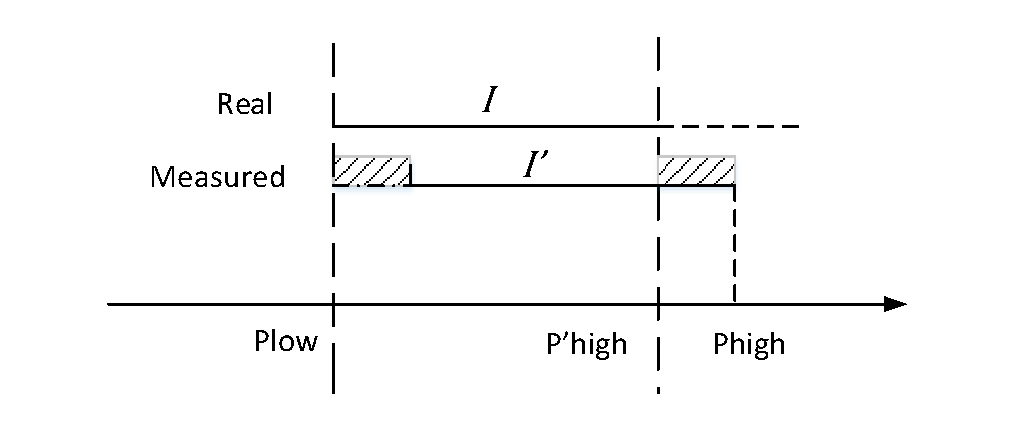
\includegraphics [width = 7cm]{Figure2.pdf}
\caption{Description.}
\label{fig:4}
\end{figure}
As shown in Figure \ref{},  we devide the physical space into many small circles each centered at $\vec r$ with radius $\vec \delta$. We assume that within each block we have a threshold  $P_{high}$ and $P_{low}$ for the RSS value$P$.  According to the $MLE$ principle used in \ref{}, which means that the probablity that the RSS falls into the ideal region must higher than the adjacent reigon, $P_{high}$ and $P_{low}$ should satisfy that 
\begin{equation}
\begin{aligned}
&f_{\vec r-\delta}(P_{high};h_{\vec r-\delta})=f_{\vec r}(P_{high};h_{\vec r})\\
&f_{\vec r+\delta}(P_{low};h_{\vec r+\delta})=f_{\vec r}(P_{low};h_{\vec r}) 
\end{aligned}
\end{equation}
. Thus we may define the reliability as the probability of the system correctly estimate the user's location,  
\begin{equation}
R = \int_{{P_{low}}}^{{P_{high}}} {{f_r}(P;h(r))dP }
\end{equation}
which means the probablity of RSS value tested in position $r$ lies within the interval $[P_{low},P_{high}]$
However, in real circumstnaces, the $P_{high}$ and $P_{low}$ are acquired through the training process, during which may recieve the imperfect data and thus cause the result to be inaccurate.The speculated location of the RSS value may migrate from the original one, causing that the RSS value from one certain region may falsely be recognized to other area. \\
 A very obvious situaiton as shown in Figure\ref{}. We assume that the deviation of the RSS value is $d$, and the current collected RSS data is $P$. We use $P'_{high}$ to denote the threshold deduced by $R$ and $P_{high}$ to denote the ideal threshold. Obviously, $P_{high}=P'_{high}-d$. The probability that the user can be mistakenly located using the data $P$ equals the probability that the user's RSS data $x$ lies within the interval of $[d,P'_{high}]$. We thus give this probability to define the error of the RSS data we collected.
\begin{equation}
\begin{aligned}
Pr_{\vec r}(error) &=\int_{P'_{high}-|d|}^{P'_{high}}f_{\vec r}(x;h(P))dx
\end{aligned}
\end{equation}
\subsection{The analysis of the loss}
We can observe from \ref{} that the error is a function of $d$, the deviation value of RSS, according to our assumption that the hypothesis $h$ is continuous function of $\mu$. We can rewrite the probability of error as the function of $h$ 
\begin{equation}
P_{\vec r}(error)=Err(|h_{\vec r}(P)-h_{\vec r}(\mu^*)|)
\end{equation}
, where $\mu^*$ is the real mean RSS value and $h_{\vec r}(\mu^*)$ is the ideal hypothesis , e.g. the real mean value of RSS when $h(x)=x$. We then use $h^*$ to denote $h_{\vec r}(\mu^*)$ and $h$ to denote$h_{\vec r}(\mu)$ for simplicity. Obviously $\mu^*$ should satisfy that 
\begin{equation}
\mu^*=arg\min_{mu\in R}E_P(Err(|h(P)-h(\mu)|))
\end{equation}
, where we defnie the $|h(P)-h(\mu)|$ as $klnf(P;h))$. The following theorem shows the rationality for our definition of error.
\begin{theorem}
The expectation of the error $Err(|h(P)-h(\mu)|)$ over $P$ get its minimum when $\mu$ equals real RSS value $\mu^*$. 
\end{theorem}
\begin{IEEEproof}
%Since that $h$ is the continuos function of $\mu(r)$, we first set that
%, where $P$ is the speculated mean value of the RSS data in $\vec r$.
\[E_P[Err(kln(f(P;h)))]\geq E_P[Err(-klnf(P;h^*))] \]
\[E_P[Err(kln(f(P,h)))]-Err(klnf(P;h*))]\geq 0\]
according to the Lagrange interpolation formula , there exists $\xi$,such that
\begin{equation*}
\begin{aligned}
&E_P[Err(kln(f(P;h)))]-h(klnf(P;h^*))]\\
=&E_P[Err'(\xi)kln(\frac{f(P;h)}{f(P;h^*)})]
\end{aligned}
\end{equation*}
obviously, $h(\xi)\>0$, consider the monotony and continuity of $Err$,there exists a minimum $m>0$ of $Err$, thus we have
\[E[h'(\xi)kln\frac{f(P;h)}{f(P;h^*)}]\geq E_P[mkln\frac{f(P;h)}{f(P;h^*)}]\]
According to Jessen inequality
\begin{equation*}
\begin{aligned}
mkE_P[ln\frac{f(P;h)}{f(P;h^*)}]&\geq mkln(E_P[ln\frac{f(P;h)}{f(P;h^*)})\\
&=mkln(\int_P\frac{f(P;h)}{f(P;h^*)}f(P;h*)dP)\\
&=mkln1=0\\
\end{aligned}
\end{equation*}
\end{IEEEproof}
Assume that we sample $N$ data $x_1,...,x_N$, we let $h*$ be the value that that minimize the $\frac{1}{N}\sum_{i=1}^N f(x_i;h)$.The theorem \ref{} above shows that when the number of data we collected is enough, the $t*$ we obtain from the data will approximate to the real RSS value $r$. We will use Hoeffding inequality to show the performance of the approximation
\begin{theorem}
The average error of $\hat{t}$ obtained from collected sample has at least $1-2e^{-\frac{2\epsilon^2}{N}}$ the probablity that is within $\epsilon$ close to the average error of real RSS data $r$, that is
\begin{equation}
Pr(\frac{1}{N}\sum_{i=1}^Nf(x_i;\hat{t})-E[f(x_i;r)]\leq\epsilon)\geq1-2e^{-\frac{2\epsilon^2}{N}}
\end{equation}
\end{theorem}
\begin{IEEEproof}
We use $Err(P;h)$ to represent $Err(klnf(P;h))$ Assume that $Err(P;h)\in[m,M]$, and in fact $0\leq m\leq M\leq 1$
according to Hoeffding inequality, for any $t$
\begin{equation*}
Pr(|\frac{1}{N}\sum_{i=1}^NErr(P;h)-E_P[Err(P;h)]|\geq \epsilon)\leq e^{-\frac{2\epsilon^2}{N}}
\end{equation*}
Assume that $\hat{h}$is our speculated hypothesis, and $h^*$is the real hypothesis, thus
\begin{equation*}
\begin{aligned}
&Pr(\frac{1}{N}\sum_{i=1}^NErr(P;\hat{h})\leq E_P[Err(P;\hat{h})+\epsilon)\geq e^{-\frac{2\epsilon^2}{N}}\\
&Pr(\frac{1}{N}\sum_{i=1}^NErr(P;h^*)\geq E_P[Err(P;h^*))-\epsilon)\geq e^{-\frac{2\epsilon^2}{N}}\\
\end{aligned}
\end{equation*}
Considering that those two events in $Pr(\dot)$ is independent to each other
\begin{equation*}\label{key}
\begin{aligned}
&Pr(\frac{1}{N}\sum_{i=1}^NErr(P;\hat{h})\leq E_P[Err(P;\hat{h}+\epsilon,\\
&\frac{1}{N}\sum_{i=1}^NErr(P;h^*))\geq E_P[Err(Ph^*))-\epsilon)\\
&\geq(1-e^{-\frac{2\epsilon^2}{N}})^2\geq 1-e^{-\frac{2\epsilon^2}{N}}\\
\end{aligned}
\end{equation*}
Since that when
\begin{equation*}
\begin{aligned}
&\frac{1}{N}\sum_{i=1}^NErr(P;\hat{h})\leq -E_P[Err(P;\hat{h}+\epsilon\\
&\frac{1}{N}\sum_{i=1}^NErr(P;h^*)\leq -E_P[Err(P;\hat{h})-\epsilon)
\end{aligned}
\end{equation*}
We have that
\begin{equation*}
\begin{aligned}
0&\leq\frac{1}{N}\sum_{i=1}^NErr(P;\hat{h})\leq -E_P[Err(P;\hat{h}\\
&\leqq\frac{1}{N}\sum_{i=1}^NErr(P;\hat{h})-Err(P;h^*)+\epsilon\\
&\leq\epsilon
\end{aligned}
\end{equation*}
Combining the equation \ref{key}, we thus have
\begin{equation}
Pr(\frac{1}{N}\sum_{i=1}^Nf(x_i;\hat{t})-E[f(x_i;r)]\leq\epsilon)\geq1-2e^{-\frac{2\epsilon^2}{N}}
\end{equation}
\end{IEEEproof}
The result shows that when $N$ is big enough, the probability that the $\hat{h}$ is close to $h^*$ will approximate to 1.
\subsection{Example of Gaussian Distribution}
We may now give a more specific example of the theories we deduce above.We assume that the RSS value $P$ folllow the Gaussian distribution with mean value of $\mu_{r}$ and variance$\sigma$. In this case, the hypothesis $h$ is exactly the mean value $\mu$. According to many previous studies\ref{}, we assume that the $\mu_{\vec r}$ is coninuous over $\vec r$. Given the fact that the $\delta$ is far smaller than $|\vec r|$, we may make an approximation that, for any position $\vec r'$ on the circle centered at $A$ with arbitrary radius $\delta$ in Figure \ref{}
\begin{equation}
\mu(\vec r')=\mu(r)+\nabla \mu(\vec r)\delta cos(\phi)
\end{equation}
, where $\phi$ is the angle between $\vec r$ and $\nabla \mu(\vec r)$. Now we consider the threshold of the RSS value. We can see from Firgure \ref{} that the threshold of the RSS is corresponding to the physical boundrary of the circle, the point B,C,D,E. Thus we can give the specific form of these two threshold.
\begin{equation}
\begin{aligned}
{P_{high}} = \mu (\vec r) + \frac{{\nabla\mu\delta \min \left\{ {\cos \phi ,\sin \phi } \right\}}}{2}\\
{P_{low}} = \mu (\vec r) - \frac{{\nabla\mu\delta \min \left\{ {\cos \phi ,\sin \phi } \right\}}}{2}
\end{aligned}
\end{equation}
Thus we may deduce the specific form of the error we defined above
\begin{equation}
\begin{aligned}
Perror(P;\vec r,\mu) &=\int_{ \mu (\vec r) + \frac{{\nabla\mu\delta \min \left\{ {\cos \phi ,\sin \phi } \right\}}}{2}}^{P (\vec r) + \frac{{\nabla P \delta \min \left\{ {\cos \phi ,\sin \phi } \right\}}}{2}}\frac{1}{\sqrt{2\pi}\sigma}e^{-\frac{(x-P)^2}{2\sigma^2}}dx
\end{aligned}
\end{equation}
Further, we can derive the form 

\section{Low-cost data purchasing problem}\label{probdef}
In this section, we will give some preliminary about the task of our mechanism and prevailing principle used in statistical machine learning. We abstractly define the problem of the designing of the effective mechanism to acquire the RSS information collected by the crowds. 

\subsection{Preliminaries}
We first give the concept of loss and regret. The loss function that reflects the data quality is defined in the space $H\times Z\to R$, where $H$ is the hypothesis class and $Z$ is the space of the objects. We expect the loss function to get its minimum value when the data is exactly the ideal data. The above theorem \ref{} has shown that the error of localization caused by the imperfectness of data we defined in\ref{} is the ideal choice. In our setting, the hypothesis $h$ is the parmeter of the probability distribution function of the RSS data in location $\vec r$. For simplicity, we denote that in each time $t$ at location $\vec r$
\begin{equation}
L_t(h_t)=Perror(P\vec r )
\end{equation}
 The $R$ is the value of After we acquire the loss function, we give the concept of the regret function.
\begin{equation}\label{def:reg}
R(T)=\sum_{t=1}^TL_t(h_t)-\min_{h^*\in H}\sum_{t=1}^TL_t(h^*_t)
\end{equation}
where $h^*$ is the optimal choice, causing the least loss in our solution space $H$. The regret function reflexes how the data deviate from the desired value, the real mean and variance of RSS. We also make some assumptions for this problem
\begin{enumerate}
\item the costs of the RSS data is arbitrarily given and have nothing to do with the data quality
\item the agents do not fabricate the data
\item the meachnism only pay at most $M$ to each data
\end{enumerate}
The reason that we make such assumptions are rather straightforward, since most people in the crowdsensing acquire the data through unprofessional devices and they do not have the ability to know the quality of their data, so they may give the price at their will. 

\subsection{Online Gradient Descent}
Online learning is a widely used learning paradign. The goal of online learning is to produce the best hypothesis when data is in sequential order
We here use the classical Online Gradient Descent(OGD) algorithm to work as the Online Algorithms. It has been proved that the OGD has an upper bound of regret of $O(\sqrt{T})$, which ensures that the average regret tends to zero when $T$ goes to infinite. There are also many kinds of other Online Algorithms which can be found in ref{OLServey}, etc. The OGD is described as following. In each time $t$, we obtain a $h_t$ according to
\begin{equation}
h_t=h_{t-1}-\eta \nabla f_t(h_{t-1})
\end{equation}.



\subsection{Importance Weighting technique}

In tradational online learning problem, all the data will be used to produce the total regret. In our low-cost purchasing problem, the mechanism do not get access to data and obtain a loss in each time $t$.  the estimation of loss is $E(\sum_{t=0}^T\delta_t f_t)=\sum_{t=0}^T q_t f_t$, where $\delta_t$ is the function showing whether the data is procured. However, the definition of regret in (\ref{def:reg}) still includes all the loss in each time $t$, whether it has been used or not.  In order to get an unbiased estimator of the regeret, we define
\begin{equation}
\hat{f_t}(h)=\begin{cases}{}
  \frac{f_t(h_t)}{q_t} & data\quad access\quad to\quad RPM  \\
  0 & else 
\end{cases}
\end{equation}
.With the unbiased estimator acquired, we can consider the mechanism as an OGD that recieves $\hat{f}$ in each round $t$.


\subsection{Problem definition}
We consider that the data collected through crowdsensing coming in a sequence of $d_1,,,d_T$, with each of them contains a cost $c_1,,,c_T$. We should design a pricing mechanism that can choose how much we should pay for the data. However, we have no means to know either the quality of data is good enough for localization or there will be a better one coming in the sequence. Under the framework of online machine learning, we formally define our RSS data Procure Mechanism ($RPM$) is defined as following.
\begin{definition}{}\label{def:1}
Given a sequence of data ${d_1,...,d_T}$ coming in time $1,,,,,T$ with each data possessing a posted price $c_t$, $c_t\in [0,M]$. 
\begin{enumerate}
\item The RPM post a hypthesis $h_t$ from OGD
\item The RPM post a price $p_t$ according to a distribution $G_t$ over $[0,M]$.
\item If the $p_t>c_t$ agent accepted the price, the RPM send the loss function $f(h_t)/q_t$ back to the OGD and pay for the posted price $p_t$. If $p_t<c_t$the agent rejected the price, the mechanism send a null data to the OGD . 
\end{enumerate}
The mechanism outputs a final hypothesis $\overline{h}\in H$
\end{definition}
And clearly, our kernel problem is to find the best distribution $G_t$ used for the mechanism to post its price 
\subsection{online batch to conversion}
The meachanism and online learning algorithm produces a sequence of hypothesis $h_1,,,h_T$. The main goal of our algorithm is to get the best hypothesis $\overline{h}$, the mean value and variance of RSS, from the sequence. One simple aproach is to average every hypothesis $h_t$ acquired in each time $t$.
\begin{equation}
\overline{h}=\sum_{t=1}^n h_t
\end{equation}
It has been proved that\ref{}, the expectation of loss of $\overline{h}$ is less than the optimal $h^*$ plus $R(T)/T$, that is 
\begin{equation*}
E_{f_1,,,f_T}Loss(\overline{h})\leq L(h^*)+\frac{R(T)}{T}
\end{equation*}
This means that if $O(R(T))<O(T)$, then the $\overline{h}$ will approximate to the optimal hypothesis $h^*$ as $T$ goes to infinite.
\section{The main setting: regret minimization senario}\label{mainsolution}
In this senario, the mechanism has a fixed budget. The target of the mechanism is that in each round $t$, the  produce the minimum regret defined in \ref{def:reg} . In this section, we will give the exact form of the distribution $G_t$ and the analysis of the regret bound according to this distribution. 
\subsection{Estimate the upper bound of regret}
We will find the upper bound of the regret defined in (\ref{def:reg}) produced by RPM. In normal case, the regret bound of OGD is 
\begin{equation}
\frac{||h||^2}{2\eta}+\eta \sum_{t=1}^T\nabla f_t(h_t)^2
\end{equation}
, which is a well known result. Under the importance weighting framework, we give the regret bound in the following lemma
\begin{Lemma}\label{lemma:reg}
The regret bound produced by RPM in \ref{def:1} is bounded by
\begin{equation}
R(h)\leq \frac{||h||^2}{2\eta}+\eta E(\sum_{t=1}^T\frac{\nabla f_t(h_t)^2}{q_t})
\end{equation}
\end{Lemma}
. The \ref{lemma:reg} is quite easy to be proved under our setting that the loss function $f_t$ is of strong convexity.

\subsection{Derivation of the Regeret Minimization Problem}

In each time $t$, the RPM need to post a price $p$ according to a distribution $g$ in order to get a minimum regret, we thus reduce the problem of designing a mechanism into an optimization problem
\begin{equation}
\begin{aligned}
&\min \sum_{i=1}^n \frac{{\nabla f_i}^2}{1-F_i(c_i)}\\
s.t. &\quad \sum_{i=1}^n\int_{c_i}^MxdF_i(x)\leq B
\end{aligned}
\end{equation}
where $\forall c_i,0\leq c_i\leq M$,and$F(0)=0,F(M)=1$
\begin{theorem}
The optimal solution of the optimization problem [\ref{}] is in the form 
\begin{equation}
F_t(c)=\begin{cases}
  1-\frac{\nabla f_t}{\sqrt{\lambda c-\beta}} &c\in(\frac{\nabla f_t^2+\beta}{\lambda},M]  \\
  0 & else 
\end{cases}
\end{equation}
\end{theorem}
\begin{IEEEproof}
We first give our function space $V=\{y|y(0)=0,y(M)=1\}$. And we denote our cost function as
\[M(F_1,,,F_n)= \sum_{i=1}^n \frac{\alpha_i}{1-F_i(c_i)}.\]
Then the augmented Lagrange function is derived as
\[J(F_1,,,F_n,\lambda)=M(F_1,,,F_n)+\lambda( \sum_{i=1}^n\int_{c_i}^MxdF_i(x)-B) \]
According to the Gateaux Deravative, we obtain that for $\forall \hat{F}\in V$
\[\delta J|_{F_t}(\hat{F_t}-F_t)=\int_{c_t}^M(-\frac{\alpha_t}{(1-F_t(c_t))^2}+\lambda x)(\hat{f}(x)-f(x))dx\]
if $\overline{F}$ is the local minimum, then we have
\[\delta J(\hat{F_t}-\overline{F_t})\geq 0\]
holds for every $\hat{F}\in V$.Noticing that
\[\int_0^Mf_t(x)-f(x)dx=0\]
We must have 
\[-\frac{\alpha_t}{(1-F_t(c_t))^2}+\lambda x\geq 0\]
hold on every where on $[c_t,M]$
thus we obtain that
\begin{equation}
F_t(c)=\begin{cases}
  1-\frac{\nabla f_t}{\sqrt{\lambda c-\beta}} &c\in(\frac{\nabla f_t^2+\beta}{\lambda},M]  \\
  0 & else 
\end{cases}
\end{equation}
\end{IEEEproof}
One major difficulty for the  is the determination of the determination of $\beta$ and $\lambda$
Noticing that $F(x)$ is not continuous, according to Stieltjes Integral, we rewrite the constraint as following
\begin{equation*}
\begin{aligned}
&\sum_{t=1}^T(\int_{c_t}^MxdF_t(x))\\
=&\sum_{t=1}^T(\int_{c_t}^Mxf_i(x)dx+(1-F_i(M)M)\\
\leq &\sum_{t=1}^T\nabla f_t (\frac{2}{\lambda}\sqrt{\lambda M-\beta}+\frac{c_t}{\sqrt{\lambda c_t-\beta}}-\frac{2}{\lambda}\sqrt{\lambda c_t-\beta})\\
\leq &B
\end{aligned}
\end{equation*}
The Stieltjes Integral here has its practical significance. Because we assume that the cost lies between $[0,M]$, in other word, the mechanism do not accept any price higher than $M$, thus for all posted price $c$ that are higher than $M$, the mechanism will only pay $M$ instead of $c$.


Now since we get the solution of the $F_t$, the remaining work is to determine the parameters $\lambda$ and $\beta$, we go back to our initial optimizationproblem that minimize the regret bound. The Lagrangian is thus given as follows
\begin{equation}
\begin{aligned}
L(\mu,\beta,\lambda)=&\sum_t \bigg( \nabla f_t\Big( \sqrt{\lambda c_t-\beta}+\mu \big(\frac{2}{\lambda}\sqrt{\lambda M-\beta}\\
&+\frac{c_t}{\sqrt{\lambda c_t-\beta}}-\frac{2}{\lambda}\sqrt{\lambda c_t-\beta}\big)\Big)\bigg)-\mu B
\end{aligned}
\end{equation}
when $\beta$ and $\lambda$ get its optimal value, it must holds that $\partial$.
According to the complementary relaxation condition, $\mu\neq 0$, which means that the constraint condition in $\ref{}$ for the optimal solution is strict. 
To get the analytic solution of the optimal value of $\beta$ and $\lambda$ is infeasible , thus we use the numeric solution for the equation \ref{}.

\subsection{Analysis of the result}
There are many things we can learn from the form given in \ref{} and parameters $\beta$ and $\lambda$. When the parameter $\beta$ and $\lambda$ is fixed, a higher $\nabla L_t$ means a higher probability that a data is acquired, which is accordance with the definition of the gradient, the fastest direction that the current $h$ to to the ideal one. Taking the parameter $\lambda$, a smaller $\lambda$ means that the mechanism would tend to pay a high price for the data, which can be seen as the data . The parameter $\beta$ can be seen as the most dominant factor that determine the minimum price that the mechanism would pay. Generally, more succifient budget $B$ would lead to a higher $\beta$ and smaller $\lambda$. When budget $B$ gose to infinite, the $\lambda$ and $\beta$ goes to infinite

 We first simply set the $\beta=0$ for a special case. Through simple calculation, we can have an estimation of $\lambda_0$ as following
\begin{equation}
\lambda_0=\frac{T}{B}(2\theta_0-\theta)
\end{equation}
where $\theta_0=\frac{1}{T}\sum_t \nabla f_t\sqrt{M}$, $\theta=\frac{1}{T}\sum_t \nabla f_t\sqrt{c_t}$
Since that $\partial L/\partial \beta >0$, $\partial L/\partial \lambda <0$, we obtain that the optimal solution $(\beta^*,\lambda^*)$ statisfy that $\beta^*>\beta^0$, $\lambda^*<\lambda_0$ Thus we have the estimate of the upper bound of the regret of RPM in theorem \ref{thm:reg-bnd}.
\begin{theorem}\label{thm:reg-bnd}
For a fixed $\beta$, the regret of RPM produced by the algorithm in \ref{} is bounded by
\begin{equation}
Regret<O(\frac{T}{\sqrt{B}}(2\theta_0-\theta)\sqrt{1-\frac{\beta B^2}{T\theta^2}})
\end{equation}

\end{theorem}
\begin{IEEEproof}

\end{IEEEproof}
One problem in this situation is that we may not get enough prior knowledge to both $c_t$ and $\nabla f_t$. One way to solve the problem is that we initially set $\beta$ to a fixed value and $\lambda$ to a very small value, e.g. $0.0001$.  Then in each time $t$, we update the value of $\lambda$ with 
\begin{align}
&\theta_0^{(t)}=\sum_{i=1}^{t-1}\frac{\nabla f_t(h_t)}{t-1}\sqrt{M}\\
&\lambda^{(t)}=\frac{T^2}{B^2M}\theta_0^2+\frac{\beta}{M}
\end{align}


\section{The budget minimization senario}
In this senario, we consider the situation that the main purpose of the mechanism is to find a strategy that can achieve  . According to most money-saving way to acquire the data inorder to achieve a satisfactory regret bound $R$. One can easily observe that ths problemThe objective function is in the form of a integral, which is not an easy problem of the classical optimization problem. Besides, to solve the very exact form of the budget do not make sense. Thus we use the aproximation of the budget B as following
\begin{equation}
\sum_t c_t q_t \leq B \leq \sum_t Mq_t
\end{equation}
\begin{theorem}
\end{theorem}
\begin{equation}
\begin{aligned}
&\min_{q_t} \sum_tc_tq_t\\
s.t. &\sum_t \frac{\nabla f_t^2}{q_t}\leq R\\
	&0\leq q_t \leq 1
\end{aligned}
\end{equation}
\subsection{The optimal mechanism}
We give our mechanism as the following theorem

\begin{IEEEproof}
Consider the convexity of the objective function, we give the Lagrangian
\begin{equation}
L=\sum_t c_t q_t -\lambda(-\sum_t\frac{\nabla f_t^2}{q_t}+R-\sum_t\mu_t(1-q_t))
\end{equation}
The optimal K-T condition of the problem \ref{} is 
\begin{align}
\frac{\partial L}{\partial q_t}=c_t-\lambda[\frac{\nabla f_t^2}{q_t^2}]-\mu_i=0
\end{align}
when $q_t=1$, we get $u_i\neq 0$, when $q_t\neq 1$, $\mu_i=0$, thus we have
\begin{equation}\label{BC:q}
q_t=\min\{1,\sqrt{\frac{\lambda}{c_t}}\nabla f_t\}
\end{equation}
According to our constraint condition
\begin{equation}
\sum_t \sqrt{\frac{c_t}{\lambda}}\nabla f_t\leq R
\end{equation}
we can get an approximation of the $\sqrt{\lambda}$ through simple calculation
\begin{equation}
\sqrt{\lambda}=\frac{T}{R}\theta
\end{equation}
where we use $\theta$ to denote the term $\frac{1}{T}\sum_t\sqrt{c_t}\nabla f_t$.
Since \ref{BC:q} holds for $\forall c_t$, and $c_t$ is arbitrarily given.We may assume that the convoluted distribution function of the price mechanism is of the form 
\begin{equation}
F_t(c)=1-\sqrt{\frac{\lambda}{c}}\nabla f_t
\end{equation}
And the PDF is 
\begin{equation}
f(c)=\frac{1}{2}\sqrt{\frac{{\lambda}}{c^3}}\nabla f_t
\end{equation}
\end{IEEEproof}
\subsection{result analysis}
Now we can make a relatively more precise estimate the budget $B$
\begin{align}
E(B)&=\sum_t\int_{c_t}^Mcf(c)dc\\
&=\frac{T^2}{R}\theta\varphi
\end{align}
where $\varphi=\sum_t\frac{1}{T}\nabla f_t(\sqrt{M}-\sqrt{c_t})$. Analogous to the \ref{}, in each round $t$, we set $\theta^{(t)}$ and $\phi^{(t)}$.


\section{Experiments and Simulations}\label{exp&sim}
In this section, we conduct the experiments and simulations to validate the performance of our system model and data procurement mechanism. We use the data collected in FoxCom Shanghai,where we tested the RSS value of 10 AP in 13 different locations, the distribution of the location and AP points are shown in Figure\ref{}. Since that the workers collected our data did not ased for reward to us, we simply simulate the costs of the data through a normal distribution with mean value of $0.5$ and variance of $1$.
\begin{figure}[htbp]
\centering
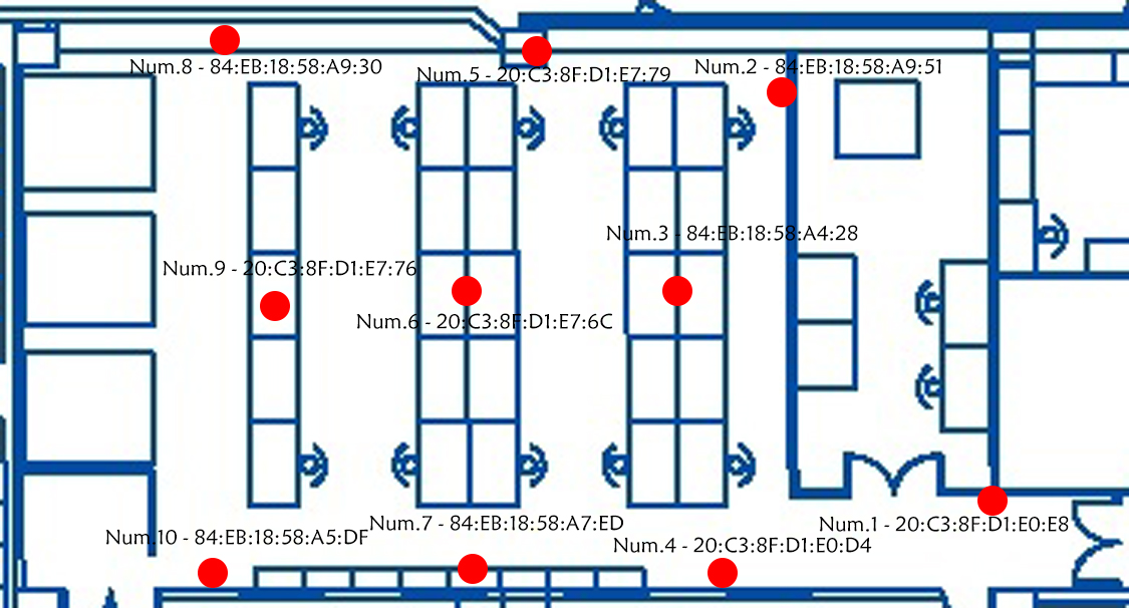
\includegraphics[width =230pt ,keepaspectratio ]{exp-loc.png}
\caption{Location Description.}
\label{fig:exp-loc}
\end{figure}

\section{Conclusion and Future Work}\label{concandfuture}


\bibliographystyle{IEEEtran}


%\bibliography{bibi}

\begin{thebibliography}{99}

\bibitem{rsscsi}
Z.~Yang, Z.~Zhou and Y.~Liu, ``From RSSI to CSI: Indoor localization via channel response,'' \emph{ACM Comput. Surv.}, vol.~46, no.~2, pp.1-32, 2013.

\bibitem{mobicom04}
A.~Haeberlen, E.~Flannery, A.~M. Ladd, A.~Rudys, D.~S. Wallach and L.~E. Kavraki, ``Practical robust localization over large-scale 802.11 wireless networks,'' in \emph{Proc. ACM MobiCom}, 2004, pp. 70--84.

\bibitem{horus}
M.~Youssef and A.~Agrawala, ``The horus wlan location determination system,'' in \emph{Proc. ACM MobiSys}, 2005, pp. 205--218.

\bibitem{wen2015fundamental}
Y.~Wen, X.~Tian, X.~Wang and S.~Lu, ``Fundamental limits of RSS fingerprinting based indoor localization,'' in \emph{Proc. IEEE INFOCOM}, 2015, pp. 2479--2487.

\bibitem{Chenshu14}
C.~Wu, Z.~Yang and Y.~Liu, ``Smartphones based Crowdsourcing for Indoor Localization,'' \emph{IEEE Transactions on Mobile Computing }, vol.~13, no.~10, pp.2199-2214, Oct. 2013.

\bibitem{luo2014piloc}
C.~Luo, H.~Hong and C.~M. Chan, ``PiLoc: a self-calibrating participatory indoor localization system,'' in \emph{Information Processing in Sensor Networks, IPSN-14 Proceedings of the 13th International Symposium on}, 2014, pp. 143--153.

\bibitem{shen2013walkie}
Shen.~G, Chen.~Z, Zhang.~P, et al. ``Walkie-Markie: indoor pathway mapping made easy[C]//Proceedings of the 10th USENIX conference on Networked Systems Design and Implementation,'' USENIX Association, 2013: 85-98.

\bibitem{ez10}
K.~Chintalapudi, A.~Padmanabha~Iyer and V.~N. Padmanabhan, ``Indoor
  localization without the pain,'' in \emph{Proc. ACM MobiCom}, 2010, pp.
  173--184.

\bibitem{Chintalapudi10}
K.~Chintalapudi, A.~Padmanabha~Iyer and V.~N. Padmanabhan, ``Indoor
  localization without the pain,'' in \emph{Proc. ACM MobiCom}, 2010, pp. 173--184.

\bibitem{ganti2011mobile}
R.~K. Ganti, F.~Ye and H.~Lei, ``Mobile crowdsensing: current state and future challenges,'' \emph{IEEE Communications Magazine}, vol.~49, no.~11, pp.32-39, 2011.

\bibitem{han2016posted}
K.~Han, H.~Huang and J.~Luo, ``Posted pricing for robust crowdsensing,'' in \emph{Proceedings of the 17th ACM International Symposium on Mobile Ad Hoc Networking and Computing}, 2016, pp. 261--270.

\bibitem{kawajiri2014steered}
R.~Kawajiri, M.~Shimosaka and H.~Kashima, ``Steered crowdsensing: Incentive design towards quality-oriented place-centric crowdsensing,'' in \emph{Proceedings of the 2014 ACM International Joint Conference on Pervasive and Ubiquitous Computing}, 2014, pp. 691--701.

\bibitem{cheung2015distributed}
M.~H. Cheung, R.~Southwell, F.~Hou and J.~Huang, ``Distributed time-sensitive task selection in mobile crowdsensing,'' in \emph{Proceedings of the 16th ACM International Symposium on Mobile Ad Hoc Networking and Computing}, 2015, pp. 157--166.

\bibitem{reddy2010recruitment}
S.~Reddy, D.~Estrin and M.~Srivastava, ``Recruitment framework for participatory sensing data collections,'' in \emph{International Conference on Pervasive Computing}, 2010, pp. 138--155.

\bibitem{lbs2}
Y.~Wen, J.~Shi, Q.~Zhang, X.~Tian, Z.~Huang, H.~Yu, Y.~Cheng and X.~Shen, ``Quality-driven auction-based incentive mechanism for mobile crowd sensing,'' \emph{IEEE Transactions on Vehicular Technology}, vol.~64, no.~9, pp.4203-4214, 2015.

\bibitem{jin2015quality}
H.~Jin, L.~Su, D.~Chen, K.~Nahrstedt and J.~Xu, ``Quality of information aware incentive mechanisms for mobile crowd sensing systems,'' in \emph{Proceedings of the 16th ACM International Symposium on Mobile Ad Hoc Networking and Computing}, 2015, pp. 167--176.

\bibitem{peng2015pay}
D.~Peng, F.~Wu and G.~Chen, ``Pay as how well you do: A quality based incentive mechanism for crowdsensing,'' in \emph{Proceedings of the 16th ACM International Symposium on Mobile Ad Hoc Networking and Computing}, 2015, pp. 177--186.

\bibitem{gao2015providing}
L.~Gao, F.~Hou and J.~Huang, ``Providing long-term participation incentive in participatory sensing,'' in \emph{2015 IEEE Conference on Computer Communications (INFOCOM)}, 2015, pp. 2803--2811.

\bibitem{abernethy2015low}
J.~Abernethy, Y.~Chen, C.~J. Ho, and B.~Waggoner, ``Low-cost learning via active data procurement,'' in \emph{Proceedings of the Sixteenth ACM Conference on Economics and Computation}, 2015, pp. 619--636.

\bibitem{yang2012locating}
Z.~Yang, C.~Wu and Y.~Liu, ``Locating in fingerprint space: wireless indoor localization with little human intervention,'' in \emph{Proceedings of the 18th annual international conference on Mobile computing and networking}, 2012, pp. 269--280.

\bibitem{wu2015smartphones}
C.~Wu, Z.~Yang and Y.~Liu, ``Smartphones based crowdsourcing for indoor localization,'' \emph{IEEE Transactions on Mobile Computing}, vol.~14, no.~2, pp.444-457, 2015.

\bibitem{walkie}
G.~Shen, Z.~Chen, P.~Zhang, T.~Moscibroda and Y.~Zhang, ``Walkie-Markie: Indoor pathway mapping made easy,'' in \emph{Proc. USENIX NSDI}, 2013, pp. 85–-98.

\bibitem{zhang2015incentivize}
Q.~Zhang, Y.~Wen, X.~Tian, X.~Gan and X.~Wang, ``Incentivize crowd labeling under budget constraint,'' in \emph{2015 IEEE Conference on Computer Communications (INFOCOM)}, 2015, pp. 2812--2820.

\bibitem{tham2015quality}
C.~K. Tham and T.~Luo, ``Quality of Contributed Service and Market Equilibrium for Participatory Sensing,'' \emph{IEEE Transactions on Mobile Computing}, vol.~14, no.~4, pp.829-842, 2015.

\bibitem{shalev2011online}
S.~Shalev-Shwartz, ``Online learning and online convex optimization,'' \emph{Foundations and Trends in Machine Learning}, vol.~4, no.~2, pp.107-194, 2011.

\bibitem{zinkevich2003online}
M.~Zinkevich, ``Online convex programming and generalized infinitesimal gradient ascent,'' School of Computer Science, Carnegie Mellon University, 2003.

\bibitem{liberzon2012calculus}
D.~Liberzon, ``Calculus of variations and optimal control theory: a concise introduction,'' Princeton University Press, 2012.

\bibitem{roth2012conducting}
<<<<<<< HEAD
A.Roth, and G.Schoenebeck, ``Conducting truthful surveys, cheaply,'' in \emph{Proceedings of the 13th ACM Conference on Electronic Commerce}, 2012, pp.826--843.

\bibitem{}

=======
A.~Roth and G.~Schoenebeck, ``Conducting truthful surveys, cheaply,'' in \emph{Proceedings of the 13th ACM Conference on Electronic Commerce}, 2012, pp.826--843.
>>>>>>> 7f9a707dc9c023d6aa376ae8f39b02d28015770e

\end{thebibliography}

\end{document}
